\documentclass[12pt, a4paper]{article}
\usepackage{ctex}

%\setCJKmainfont[ItalicFont={AR PL UKai CN}]{AR PL UMing CN}
%\setCJKsansfont{WenQuanYi Zen Hei}
%\setCJKmonofont{WenQuanYi Zen Hei Mono}

\setcounter{secnumdepth}{0}
\usepackage[margin=1.5in]{geometry}
\usepackage{color}
\usepackage{clrscode}
\usepackage{amssymb}
\usepackage{amsthm}
\usepackage{amsmath}
\definecolor{bgGray}{RGB}{36, 36, 36}
\usepackage{supertabular}
\usepackage[
  colorlinks,
  linkcolor=bgGray,
  anchorcolor=blue,
  citecolor=green
]{hyperref}
\usepackage{listings}
\usepackage{fontspec}
\newfontfamily\courier{Courier}
\usepackage{xcolor}
\title{想法与解答}
\author{吴章昊}
\begin{document}
\bibliographystyle{plain}
\lstset{numbers=left,
  basicstyle=\scriptsize\courier,
  numberstyle=\tiny\courier\color{red!89!green!36!blue!36},
  language=Python,
  breaklines=true,
  keywordstyle=\color{blue!70},commentstyle=\color{red!50!green!50!blue!50},
  morekeywords={},
  stringstyle=\color{purple},
  frame=shadowbox,
  rulesepcolor=\color{red!20!green!20!blue!20}
}
\maketitle
\tableofcontents
\newpage
\section{解答}
\subsection{对角线旅行}
\subsubsection{问题描述}
在一个大方格内,从(0,0)出发,通过抛硬币决定每次是向右移动一个单位还是向上移动一个单位。在能够到达(n,n)位置的所有路线中,对角线上方出现的向上移动的个数为0,1,2...,n时,概率分别为多少?
\subsubsection{解答}
\begin{figure}[htbp]
    \centering
    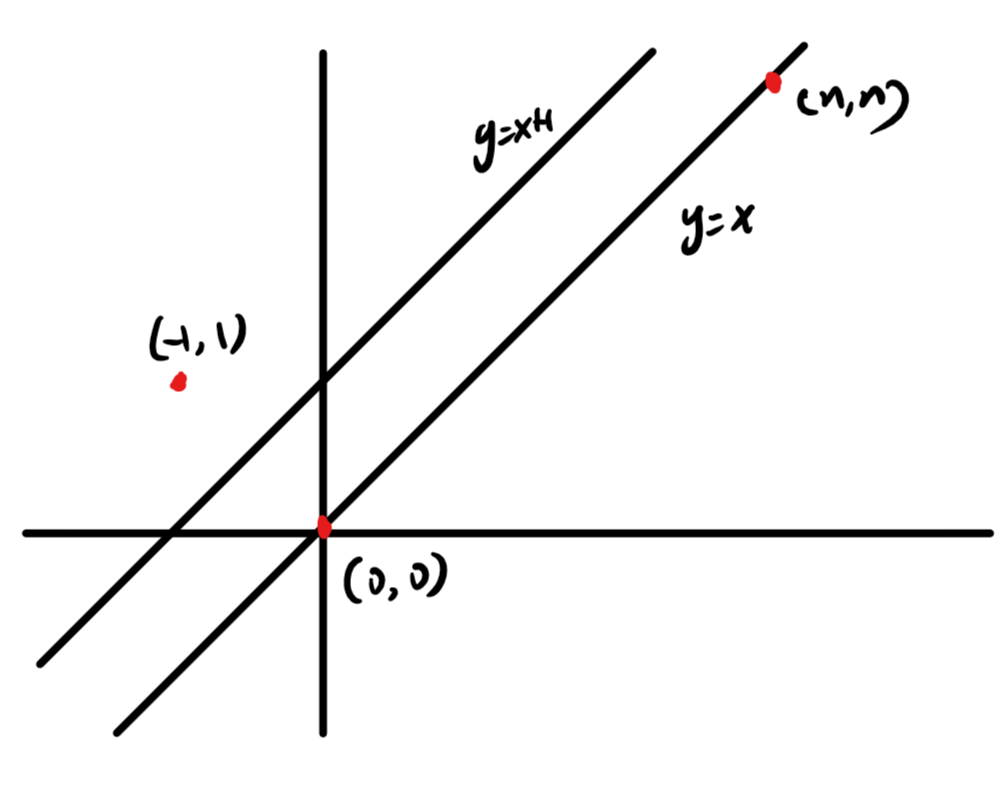
\includegraphics[width=3in]{../resource/diagonal.png}
    \caption{对角线旅行}
\end{figure}
令函数$N(k,u)$,为从(0,0)到(k,k)的路线中对角线上方出现向上移动数目为u的路线总数
\begin{enumerate}
    \item 首先考虑,所有的向上移动都在对角线下方的情况。\par
    先计算,有通过对角线的路径。对于这种路径,它必然会与$f(x) = y = x + 1$相交,那么,假设它与$f(x)$的第一个交点为P,将P之前的路径关于$f(x)$做对称,可以得到从(-1,1)到(n,n)的路径,而由于要从(-1,1)到(n,n)并定会与$f(x)$相交,所以,从(-1,1)到(n,n)的路径总数即为从(0,0)到(n,n)的路径中穿过对角线的数目,即$\binom{2n}{n-1}$。\par
    则所有向上移动都在对角线下方的路径数目为$N(n,0)=\binom{2n}{n}-\binom{2n}{n-1} = \frac{1}{n+1}\binom{2n}{n}$。\cite{Diagonal_travel}\par
    \item 现在,利用数学归纳法证明,$\forall t\in[0,k], N(k,t)=\frac{1}{k+1}\binom{2k}{k}=C_k$, where $t \leq k$
    \begin{itemize}
        \item 对于k=1,2是显然结论是成立的
        \item 对于$k \geq 2$,假设$k=1,2...,m$结论均成立,讨论路径与对角线第一次相交前的向上移动的数目s,前s的路径数为$N(s-1,0)$或$N(s-1,s-1)$(均在对角线上方,或均在对角线下方),则对于$k=m+1$有递推公式,
        \begin{displaymath}
            \begin{aligned}
                N(k,t)&=\sum^{k-t}_{s=1}{N(s-1,0)N(k-s,t)}\\&\text{ \ \ }+\sum^{t}_{s=1}{N(s-1,s-1)N(k-s,t-s)}\\
                    &=\sum^{k-t-1}_{p=0}{N(p,0)N(k-1-p,t)}\\&\text{ \ \ }+\sum^{t-1}_{p=0}{N(p,0)N(k-1-p,t-p-1)}\\
                    &=\sum^{k-t-1}_{p=0}{C_pC_{k-1-p}}+\sum^{t-1}_{p=0}{C_pC_{k-1-p}}\\
                    &=\sum^{k-t-1}_{p=0}{C_pC_{k-1-p}}+\sum^{k-1}_{p=k-t}{C_{k-1-p}C_p}\\
                    &=\sum^{k-1}_{p=0}{C_pC_{k-1-p}}
            \end{aligned}
        \end{displaymath}
        由Catalan number的性质有$\sum^{k-1}_{p=0}{C_pC_{k-1-p}}=C_k$        
    \end{itemize}
    得证
\end{enumerate}
因此,题中所求概率均为${C_n}/{\binom{2n}{n}}=\frac{1}{n+1}$

\subsection{掷骰子问题}
\subsubsection{改变概率}
不可能,见笔记
\subsubsection{改变表面数字}
不可能,因为在等概率的情况下,36种组合等概率,而2-12中的每个数的概率均为$\frac{1}{11}$,则每个数对应的组合为$36\times \frac{1}{11}$不是整数,矛盾!
\subsubsection{改变概率和数字}
I don't know

\section{思考}
\subsection{3个孩子的家庭}
对于这个问题的两个结果,我认为主要的原因在于对于两个家庭概率的判断并不是建立在同一个概率模型上的,对于前者,即2个男孩,1个女孩的家庭的概率是在 {所有有3个孩子的家庭} 这样的样本空间上考虑的;而对于后者是建立在样本空间:{所有有3个孩子的家庭 and 其中1个为女孩}。因此会得到两个不同的概率结果。
\subsection{Sleeping Beauty(SB)}
\begin{figure}[htbp]
    \centering
    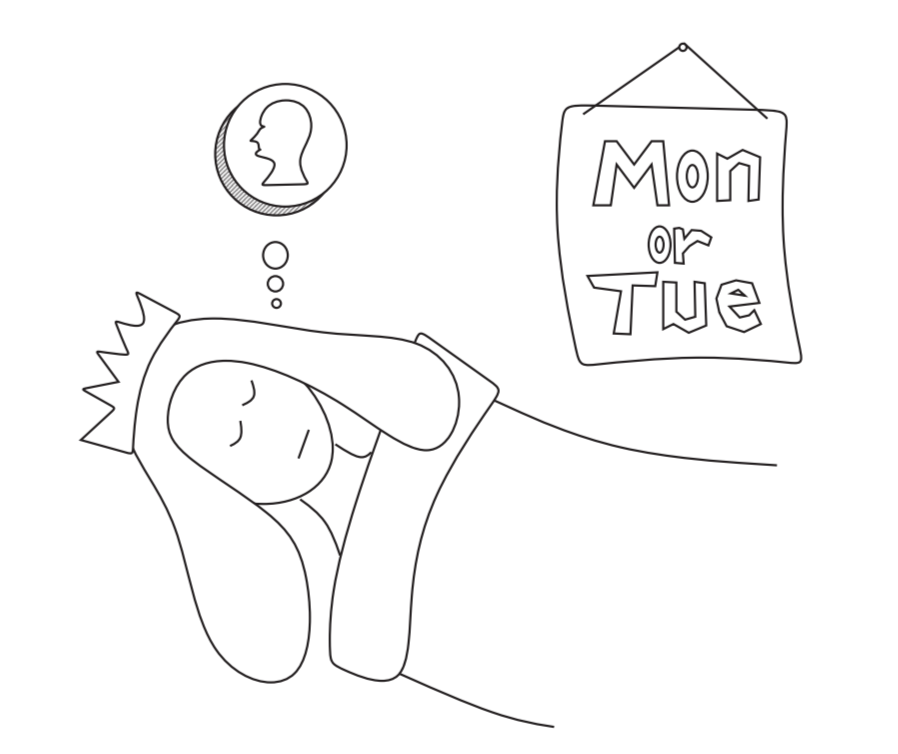
\includegraphics[width=3.5in]{../resource/SB.png}
    \caption{Sleeping beauty having a dream}
\end{figure}
关于硬币Heads的概率,论文中做了详细的讨论,将$\frac{1}{3}$的支持者“thirders”和$\frac{1}{2}$的支持者“halfers”以及一些持其他观点人的论断和依据都予以罗列。我个人还是更加认同thirders的Repetition观点。我认为对于SB而言,Tail会使她醒来两次,而Head只会让她醒来一次,这就造成了她醒来所遇到的硬币面并不是等概率的。\par
论文中提到了halfers的一种看法是,在SB睡前硬币的概率应当为$\frac{1}{2}$,而在之后的醒来中,信息量并没有增加,因此,概率不发生变化。而论文在Information revisited,thirders的反驳中提到,information应该还来源于时间是否被测量,时刻是否应该被记作一个时刻,从而表明信息量发生了变化。但是,我认为也许原本周日时SB预测和周一周二时的概率是两次不同的试验,前者是将硬币的正反结果作为样本空间,而后者既然是对于SB而言的就应该将周一、周二的计入到样本空间中。它们的样本空间也就存在差异,并不能直接过渡。在我看来,题目中所求的概率是对于SB而言的,对于SB,其实相当于每当硬币为Tail时,结果都会被“记录”两次,而Head时只会有一次。引出的结论应和均等的记录正反面不同。\par
对于这篇论文最后所提到的一些内容,我还存在一些疑问。Optional Stopping Theorem关于下雪天的概率描述,按照我的理解是将时间要素考虑在内,也就是随着时间的迁移,learning增加使得概率发生变化。我感到有一些困惑。对于下雪天的这个例子,在一个密闭的环境下,试验的结果应该只反映在7点那一个时刻上,在之前的时刻中,钟声必定不会响起,那么概率的不断减小究竟如何与时间建立定量的联系呢?

\bibliography{./Thoughts_ZhWu}

\end{document}

